\documentclass[a4paper,twoside,openany]{report}

\usepackage[a4paper,top=3cm,bottom=3cm,left=3cm,right=3cm]{geometry}
\usepackage[fontsize=13pt]{scrextend}
\usepackage[english]{babel}
\usepackage[T1]{fontenc}
\usepackage[utf8]{inputenc}
\usepackage{lmodern}
\usepackage{microtype}
\usepackage{amsmath}
\usepackage{graphicx}
\usepackage{hyperref}

\hypersetup{
    colorlinks,
    linkcolor=black,
    citecolor=black,
    urlcolor=black
}

\pagestyle{plain}

\begin{document}

\begin{titlepage}

\begin{figure}[!htb]
\centering

\includegraphics[keepaspectratio=true,scale=0.5]{Images/cherubinFrontespizio.eps}
\end{figure}

\begin{center}
    \LARGE{UNIVERSITY OF PISA}
    \vspace{5mm}
    \\ \large{DEPARTMENT OF INFORMATION ENGINEERING}
    \vspace{5mm}
    \\ \LARGE{Master's Degree in Robotics and Automation Engineering}
\end{center}

\vspace{15mm}
\begin{center}
    {\LARGE{\bf Navigation System Project}}
    \\ {\bf Navigation System Design for HAPS Drone}
\end{center}

\vspace{30mm}

\begin{minipage}[t]{0.47\textwidth}
    {\large{Supervisor:}{\normalsize\vspace{3mm}
    \bf\\ \large{Prof. Lorenzo Pollini}}}
\end{minipage}
\hfill
\begin{minipage}[t]{0.47\textwidth}\raggedleft
    {\large{Candidate:}{\normalsize\vspace{3mm}
    \bf\\ \large{Rolando Giugliano}}}
\end{minipage}

\vspace{30mm}
\hrulefill
\\\centering{\large{ACADEMIC YEAR 2025/2026}}

\end{titlepage}

\cleardoublepage
\tableofcontents
\cleardoublepage

\chapter{Introduction}

The objective of this project is to design, simulate, and validate an integrated Inertial Navigation System (INS) aided by a Global Navigation Satellite System (GNSS). The system architecture, the kinematic models, and the required sensor suite were strictly dictated by a uniquely assigned project code, which outlines a specific set of algorithmic and structural specifications.

\section{Project Specifications}

The system has been developed according to the assigned code D - E - E - G/a - E - PV, which translates to the following architectural choices:

\begin{itemize}
    \item \textbf{D (Decoupled Estimation):} The navigation system features a decoupled architecture. The attitude estimation is performed separately from the position and velocity estimation, utilizing two distinct filtering instances.
    \item \textbf{E (Ellipsoid Earth Model):} The kinematic mechanization assumes an ellipsoidal Earth model (WGS84). The position state is expressed in geodetic coordinates (Latitude, Longitude, Altitude), requiring the dynamic computation of the meridian and transverse radii of curvature ($R_M$ and $R_N$).
    \item \textbf{E (Euler Angles Parameterization):} The attitude of the vehicle is parameterized within the state vector using Euler angles (Roll, Pitch, Yaw) rather than quaternions.
    \item \textbf{G/a (Sensor Bias Estimation):} The gyroscope bias is actively estimated within the filter state and fed back to correct the raw measurements. Conversely, the accelerometer bias is not estimated, relying solely on the stochastic noise model.
    \item \textbf{E (Attitude Measurements):} The attitude filter exploits direct measurements of the Euler angles, simulating the output of an Attitude and Heading Reference System (AHRS), to correct the inertial integration.
    \item \textbf{PV (Position and Velocity Measurements):} The navigation filter is aided by direct observations of both 3D position and 3D velocity, representing a typical GNSS receiver output in a loosely coupled configuration.
\end{itemize}

\section{Operational Scenario and Trajectory Generation}

To properly stress the ellipsoidal kinematics and evaluate the filter's performance over significant Earth-surface displacements, the simulated scenario must involve extended distances and high altitudes. For this reason, the chosen vehicle is a High Altitude Pseudo-Satellite (HAPS), taking the flight characteristics of the Airbus Zephyr as a realistic operational example.

The simulated mission represents a nighttime stratospheric flight with a total duration of 30 minutes (1800 seconds). The vehicle starts at a cruising altitude of 20,000 meters, flying at a highly efficient airspeed of approximately 20 m/s. Due to the massive wingspan and structural constraints typical of HAPS platforms, the generated trajectory is characterized by extremely gentle dynamics, featuring wide turning radii.

Furthermore, to accurately simulate the nighttime power-saving operation, where electric propulsion is minimized in the absence of solar irradiance, a slow and linear altitude loss of 200 meters is distributed over the 30-minute window. This specific scenario highlights the necessity of the WGS84 ellipsoidal model, as a flat-Earth approximation would introduce significant divergence over such extended operational ranges, and provides a challenging dynamic for the vertical channel of the error-state Kalman filter.

\begin{figure}[!htbp]
    \centering
    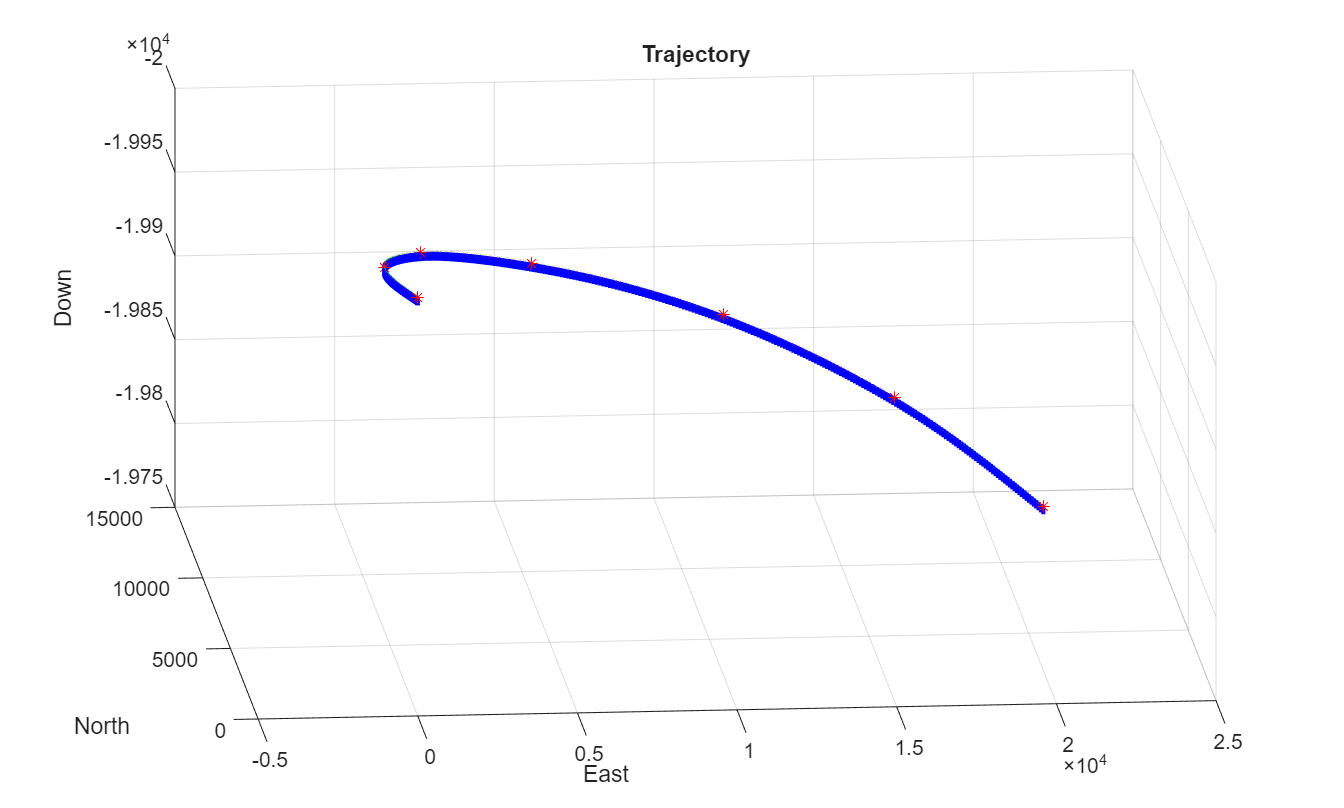
\includegraphics[width=0.9\linewidth]{Images/traj_ideal.png} 
    \caption{Simulated HAPS trajectory in NED frame.}
    \label{fig:traj_ideal}
\end{figure}

\chapter{Inertial Mechanization on the Ellipsoidal Earth}

The core of the navigation system is the mechanization algorithm, which integrates the high-frequency measurements provided by the Inertial Measurement Unit (IMU), namely specific forces and angular velocities, to track the vehicle's position, velocity, and attitude. According to the project specifications, the mechanization is formulated over the WGS84 ellipsoidal Earth model, avoiding flat-Earth approximations.

The algorithm is structured into three interconnected modules: position kinematics, attitude update with transport-rate compensation, and gravity compensation.

\section{Ellipsoidal Position Kinematics}

The vehicle's position is expressed in the geodetic coordinate frame (LLH), comprising latitude, longitude, and altitude. To avoid ambiguity with the roll angle, geodetic latitude is denoted here by $\varphi$, while longitude and altitude are denoted by $\lambda$ and $h$, respectively. Because of the oblateness of the WGS84 ellipsoid, the Earth's radii of curvature are not constant and must be evaluated as functions of the current latitude.

The prime vertical radius of curvature $R_N$ and the meridian radius of curvature $R_M$ are computed at each time step as

\begin{equation}
    R_N = \frac{R_e}{\sqrt{1 - e^2 \sin^2\varphi}}
    \label{eq:RN}
\end{equation}

\begin{equation}
    R_M = R_N \frac{1 - e^2}{1 - e^2 \sin^2\varphi}
    \label{eq:RM}
\end{equation}

where $R_e = 6\,378\,137\,\mathrm{m}$ is the semi-major axis and $e \approx 0.0818$ is the first eccentricity of the ellipsoid.

Using the navigation-frame velocities $v_N$, $v_E$, and $v_D$, the LLH kinematic time derivatives are given by

\begin{equation}
    \dot{\varphi} = \frac{v_N}{R_M + h}
    \label{eq:phi_dot}
\end{equation}

\begin{equation}
    \dot{\lambda} = \frac{v_E}{(R_N + h)\cos\varphi}
    \label{eq:lambda_dot}
\end{equation}

\begin{equation}
    \dot{h} = -v_D
    \label{eq:h_dot}
\end{equation}

These derivatives are numerically integrated to propagate the vehicle's geodetic position.

\section{Attitude Update and Transport-Rate Compensation}

The attitude of the vehicle is parameterized using Euler angles, namely roll $\phi_{\mathrm{roll}}$, pitch $\theta$, and yaw $\psi$, which represent the orientation of the body frame with respect to the local NED frame.

The raw angular velocities measured by the gyroscope, $\boldsymbol{\omega}_{ib}^b$, are referenced to the inertial frame. However, the local NED frame is not stationary: it rotates with respect to the inertial frame because of both the Earth's rotation and the motion of the vehicle over the curved Earth surface. This combined rotation is the transport rate, $\boldsymbol{\omega}_{in}^n$, defined as the sum of the Earth rate $\boldsymbol{\omega}_{ie}^n$ and the craft rate $\boldsymbol{\omega}_{en}^n$:

\begin{equation}
    \boldsymbol{\omega}_{ie}^n =
    \begin{bmatrix}
        \omega_E \cos\varphi \\
        0 \\
        -\omega_E \sin\varphi
    \end{bmatrix}
    \label{eq:omega_ie}
\end{equation}

\begin{equation}
    \boldsymbol{\omega}_{en}^n =
    \begin{bmatrix}
        \dfrac{v_E}{R_N + h} \\
        \dfrac{-v_N}{R_M + h} \\
        \dfrac{-v_E \tan\varphi}{R_N + h}
    \end{bmatrix}
    \label{eq:omega_en}
\end{equation}

\begin{equation}
    \boldsymbol{\omega}_{in}^n = \boldsymbol{\omega}_{ie}^n + \boldsymbol{\omega}_{en}^n
    \label{eq:omega_in}
\end{equation}

where $\omega_E \approx 7.2921 \times 10^{-5}\,\mathrm{rad\,s^{-1}}$ is the Earth's rotation rate.

To correctly update the vehicle's attitude, the transport rate must be projected into the body frame via the direction cosine matrix $C_n^b$ and subtracted from the raw gyroscope measurements. The corrected body angular rates are then mapped into Euler-angle derivatives using the standard kinematic Jacobian $J$:

\begin{equation}
    \begin{bmatrix}
        \dot{\phi}_{\mathrm{roll}} \\
        \dot{\theta} \\
        \dot{\psi}
    \end{bmatrix}
    =
    \begin{bmatrix}
        1 & \sin\phi_{\mathrm{roll}}\tan\theta & \cos\phi_{\mathrm{roll}}\tan\theta \\
        0 & \cos\phi_{\mathrm{roll}} & -\sin\phi_{\mathrm{roll}} \\
        0 & \dfrac{\sin\phi_{\mathrm{roll}}}{\cos\theta} & \dfrac{\cos\phi_{\mathrm{roll}}}{\cos\theta}
    \end{bmatrix}
    \left( \boldsymbol{\omega}_{ib}^b - C_n^b \boldsymbol{\omega}_{in}^n \right)
    \label{eq:euler_rates}
\end{equation}

\section{Gravity Compensation}

The accelerometers measure the specific force $\mathbf{f}^b$, which includes both the kinematic acceleration of the vehicle and the reaction to the Earth's gravitational field. To isolate the true kinematic acceleration needed for the velocity update, the gravity contribution must be subtracted.

Within the WGS84 framework, gravity is not a constant $9.81\,\mathrm{m\,s^{-2}}$. The mechanization adopts the Somigliana closed-form expression to compute the local gravity magnitude $g(\varphi)$ on the ellipsoid surface as a function of latitude:

\begin{equation}
    g(\varphi) = g_{\mathrm{wgs0}} \frac{1 + g_{\mathrm{wgs1}} \sin^2\varphi}{\sqrt{1 - e^2 \sin^2\varphi}}
    \label{eq:gravity}
\end{equation}

where $g_{\mathrm{wgs0}} \approx 9.7803\,\mathrm{m\,s^{-2}}$ is the gravity at the equator and $g_{\mathrm{wgs1}}$ is the gravity formula constant. The resulting local gravity vector is

\begin{equation}
    \mathbf{g}^n = \begin{bmatrix} 0 & 0 & g(\varphi) \end{bmatrix}^T,
    \label{eq:gravity_vector}
\end{equation}

and is transformed into the body frame and subtracted from the specific-force measurements before the velocity update.

\end{document}
